%! Author = thibaultchausson
%! Date = 11/12/2023

\subsection {Paramètres du problème}

La méthode de la colonie de fourmis étant spécialisée dans la résolution de problèmes analogues à celui du marchand de commerce, nous allons tout d'abord devoir la redéfinir pour être compatible avec notre sujet.

Il faut d'abord définir ce que représenteront les n\oe uds et les chemins du problème.

Une première approche serait de considérer chaque n\oe ud comme une configuration possible de l'emploi du temps, et chaque chemin comme le passage d'une configuration à une autre.

Cependant, cette approche s'avère rapidement irréalisable.
Chaque cours peut se trouver dans 6 configurations : assigné à un des 5 jours de la semaine, ou non-assigné.

Avec 10 cours, on atteint $6^{10} = ~6E7$ n\oe uds, ce qui, au delà des problèmes de mémoire, demanderait aux fourmis un nombre d'itérations astronomique pour faire le moindre progrès.

Il s'avère en réalité que le problème de l'affectation d'emploi du temps est assez peu compatible avec la méthode de la colonie de fourmis.
Il est néanmoins possible d'en utiliser une version modifiée.

Pour limiter le nombre de n\oe uds, on considérera 11 n\oe uds, le premier représentant l'emploi du temps initial vide, et chaque n\oe ud suivant représentant un des 10 cours à affecter.

Chaque paire de n\oe uds consécutifs sera séparée par 5 chemins, représentant les 5 jours de la semaine auxquels peut être affecté le prochain cours.

Les fourmis parcourront donc tous les n\oe uds dans le même ordre, mais en empruntant des chemins différents entre chaque n\oe ud, comme représenté sur ce graphe :

\begin{center}
    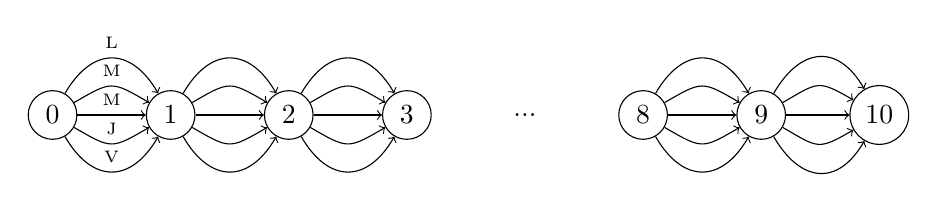
\begin{tikzpicture}[node distance={15mm}, main/.style = {circle}]
        \node[main,draw] (0) {$0$};
        \node[main,draw] (1) [right of=0] {$1$};
        \node[main,draw] (2) [right of=1] {$2$};
        \node[main,draw] (3) [right of=2] {$3$};
        \node[main  ] (...) [right of=3] {$...$};
        \node[main,draw] (8) [right of=...] {$8$};
        \node[main,draw] (9) [right of=8] {$9$};
        \node[main,draw] (10) [right of=9] {$10$};

        % Lien avec L
        \draw[->] (0) to [out=60,in=120,looseness=1.5] node[above, font=\fontsize{6pt}{7.2pt}\selectfont] {L} (1);
        % Lien avec M
        \draw[->] (0) to [out=30,in=150,looseness=1.5] node[above, font=\fontsize{6pt}{7.2pt}\selectfont] {M} (1);
        % Lien avec M
        \draw[->] (0) to node[above, font=\fontsize{6pt}{7.2pt}\selectfont] {M} (1);
        % Lien avec J
        \draw[->] (0) to [out=-30,in=210,looseness=1.5] node[above, font=\fontsize{6pt}{7.2pt}\selectfont] {J} (1);
        % Lien avec V
        \draw[->] (0) to [out=-60,in=-120,looseness=1.5] node[above, font=\fontsize{6pt}{7.2pt}\selectfont] {V} (1);


        % Autres liens (sans lettres)
        \foreach \m in {0,1,2,3,4}{
            \draw[->] (1) to [out=60-30*\m,in=120+30*\m,looseness=1.5] (2);
        }
        \foreach \m in {0,1,2,3,4}{
            \draw[->] (2) to [out=60-30*\m,in=120+30*\m,looseness=1.5] (3);
        }
        \foreach \m in {0,1,2,3,4}{
            \draw[->] (8) to [out=60-30*\m,in=120+30*\m,looseness=1.5] (9);
        }
        \foreach \m in {0,1,2,3,4}{
            \draw[->] (9) to [out=60-30*\m,in=120+30*\m,looseness=1.5] (10);
        }
    \end{tikzpicture}
\end{center}


Chaque chemin, de haut en bas, représente un jour de lundi à vendredi.

Au lieu de pondérer le choix du prochain n\oe ud par sa distance, les fourmis calculeront le nombre de conflits engendrés par le choix de chaque chemin.

Ainsi, la probabilité qu'un chemin $c$ soit choisi pour passer du n\oe ud $n-1$ au n\oe ud $n$ est décrite par la formule suivante :

$$P_{n,c} = \frac{\tau^{\alpha}_{n,c}\eta^{\beta}_{n,c}}{\sum^{5}_{d = 0}{\tau^{\alpha}_{n,d}\eta^{\beta}_{n,d}}}$$

Avec $\alpha$ et $\beta$ deux réels positifs, $\tau_{n,c}$ la trace de phéromones présente sur le chemin $c$ entre les n\oe uds $n-1$ et $n$, et $\eta_{n,c} = \frac{1}{1 + conflits_{n,c}}$, avec $conflits_{n,c}$ le nombre de classes devant assister à la fois au cours $n$, et à au moins un autre cours déjà assigné au jour $c$.

A la fin de leur parcours, les fourmis déposeront sur leur chemin une trace proportionnelle au score de fitness de l'emploi du temps obtenu, et on met à jour la trace via la formule :

$$\tau_{n,c} = (1-\rho)\tau_{n,c} + Q\sum_{k \in K}{\Delta^k_{n,c}}$$

Avec $K$ l'ensemble des fourmis, $\rho \in ]0;1[$ le facteur d'évaporation, $Q$ une constante, et $\Delta^k_{n,c}$ égal à la fitness de la fourmi $k$ si elle a emprunté le chemin $(n,c)$, et $0$ sinon.

Une fois le nombre d'itérations voulues passer, on retourne la fourmi de la population finale ayant la meilleure fitness.


\subsection{Application numérique}\label{subsec:application-numerique}

On initialise l'algorithme avec les constantes suivantes :

\begin{itemize}
    \item $\alpha = 0.5$
    \item $\beta = 0.5$
    \item $Q = 1$
    \item $\rho = 0.7$
    \item $\tau_0 = 0.001$
    \item Population de fourmis : $10$
    \item Nombre d'iterations : $3$
\end{itemize}

La première fourmi se trouve au n\oe ud $0$.
Les probabilités de choix pour le prochain chemin sont :


\begin{table}[h!]
    \centering
    \begin{tabular}{|c|c|c|c|c|c|}
        \hline
        Chemin      & 1   & 2   & 3   & 4   & 5   \\
        \hline
        Probabilité & 0.2 & 0.2 & 0.2 & 0.2 & 0.2 \\
        \hline
    \end{tabular}
    \caption{Probabilités de choix de la fourmi 1 pour le n\oe ud 1 à la génération 1}\label{tab:fourmi-1-noeud-1-gen-1}
\end{table}

Elle choisit le n\oe ud $3$.
Les probabilités de choix pour le n\oe ud 2 sont ainsi :

\begin{table}[h!]
    \centering
    \begin{tabular}{|c|c|c|c|c|c|}
        \hline
        Chemin      & 1    & 2    & 3    & 4    & 5    \\
        \hline
        Probabilité & 0.22 & 0.22 & 0.12 & 0.22 & 0.22 \\
        \hline
    \end{tabular}
    \caption{Probabilités de choix de la fourmi 1 pour le n\oe ud 2 à la génération 1}\label{tab:fourmi-1-noeud-2-gen-1}
\end{table}

La fourmi choisit le n\oe ud $1$.
On continue jusqu'au n\oe ud $10$, et on obtient le chemin suivant :


\begin{center}
    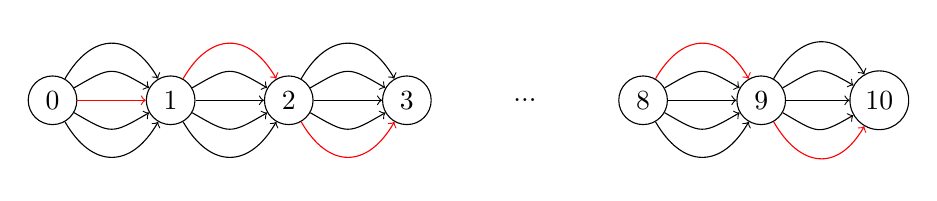
\begin{tikzpicture}[node distance={15mm}, main/.style = {circle}]
        \node[main,draw] (0) {$0$};
        \node[main,draw] (1) [right of=0] {$1$};
        \node[main,draw] (2) [right of=1] {$2$};
        \node[main,draw] (3) [right of=2] {$3$};
        \node[main  ] (...) [right of=3] {$...$};
        \node[main,draw] (8) [right of=...] {$8$};
        \node[main,draw] (9) [right of=8] {$9$};
        \node[main,draw] (10) [right of=9] {$10$};

        \foreach \m in {0,1,3,4}{
            \draw[->] (0) to [out=60-30*\m,in=120+30*\m,looseness=1.5] (1);
        }

        \draw[red, ->] (0) to [out=0,in=180,looseness=1.5] (1);

        \foreach \m in {1,2,3,4}{
            \draw[->] (1) to [out=60-30*\m,in=120+30*\m,looseness=1.5] (2);
        }

        \draw[red, ->] (1) to [out=60,in=120,looseness=1.5] (2);

        \foreach \m in {0,1,2,3}{
            \draw[->] (2) to [out=60-30*\m,in=120+30*\m,looseness=1.5] (3);
        }

        \draw[red, ->] (2) to [out=-60,in=240,looseness=1.5] (3);
        
        \foreach \m in {1,2,3,4}{
            \draw[->] (8) to [out=60-30*\m,in=120+30*\m,looseness=1.5] (9);
        }

        \draw[red, ->] (8) to [out=60,in=120,looseness=1.5] (9);
        
        \foreach \m in {0,1,2,3}{
            \draw[->] (9) to [out=60-30*\m,in=120+30*\m,looseness=1.5] (10);
        }

        \draw[red, ->] (9) to [out=-60,in=240,looseness=1.5] (10);
    \end{tikzpicture} 
\end{center}


Ce qui correspond avec la répartition suivante :

\begin{table}[H]
    \centering
    \begin{tabular}{|c|c|c|c|c|c|c|}
        \hline
        Jour  & 1       & 2 & 3          & 4 & 5        & Fitness \\
        \hline
        Cours & 2, 4, 9 &   & 1, 5, 6, 8 &   & 3, 7, 10 & 6       \\
        \hline
    \end{tabular}
    \caption{Répartition de l'emploi du temps de la fourmi 1 à la génération 1}\label{tab:fourmi-1-gen-1}
\end{table}

Après avoir répété l'opération pour les 10 fourmis, on obtient comme élite la fourmi 6 :

\begin{table}[!h]
    \centering
    \begin{tabular}{|c|c|c|c|c|c|c|}
        \hline
        Jour  & 1 & 2              & 3 & 4 & 5       & Fitness \\
        \hline
        Cours & 2 & 1, 5, 7, 9, 10 & 3 &   & 4, 6, 8 & 8       \\
        \hline
    \end{tabular}
    \caption{Répartition de l'emploi du temps de la fourmi 6 à la génération 1}\label{tab:fourmi-6-gen-1}
\end{table}

La trace de phéromones est la suivante :

\begin{table}[!h]
    \centering
    \begin{tabular}{|c|c|c|c|c|c|}
        \hline
        \diagbox{Noeud}{Chemin} & 1       & 2       & 3       & 4       & 5       \\
        \hline
        1                       & 1.0e-03 & 2.9e+01 & 1.2e+01 & 1.5e+01 & 1.4e+01 \\
        \hline
        2                       & 2.3e+01 & 1.0e+01 & 1.7e+01 & 1.4e+01 & 6.0e+00 \\
        \hline
        3                       & 1.0e-03 & 1.9e+01 & 8.0e+00 & 8.0e+00 & 3.5e+01 \\
        \hline
        4                       & 1.0e+01 & 2.2e+01 & 1.5e+01 & 7.0e+00 & 1.6e+01 \\
        \hline
        5                       & 9.0e+00 & 2.0e+01 & 1.8e+01 & 1.7e+01 & 6.0e+00 \\
        \hline
        6                       & 7.0e+00 & 1.8e+01 & 1.6e+01 & 1.0e-03 & 2.9e+01 \\
        \hline
        7                       & 1.2e+01 & 1.8e+01 & 7.0e+00 & 2.3e+01 & 1.0e+01 \\
        \hline
        8                       & 6.0e+00 & 1.2e+01 & 2.8e+01 & 7.0e+00 & 1.7e+01 \\
        \hline
        9                       & 2.0e+01 & 3.6e+01 & 1.0e-03 & 1.0e-03 & 1.4e+01 \\
        \hline
        10                      & 1.0e+01 & 3.9e+01 & 1.0e-03 & 1.0e-03 & 2.1e+01 \\
        \hline
    \end{tabular}
    \caption{Trace laissée par la génération 1}\label{tab:trace-gen-1}
\end{table}

On passe maintenant à la deuxième génération de fourmis :

La première fourmi se trouve au n\oe ud $0$.
Les probabilités de choix pour le prochain chemin sont :


\begin{table}[!h]
    \centering
    \begin{tabular}{|c|c|c|c|c|c|}
        \hline
        Chemin      & 1     & 2     & 3     & 4     & 5     \\
        \hline
        Probabilité & 0.001 & 0.326 & 0.210 & 0.235 & 0.228 \\
        \hline
    \end{tabular}
    \caption{Probabilités de choix de la fourmi 1 pour le n\oe ud 1 à la génération 2}\label{tab:fourmi-1-noeud-1-gen-2}
\end{table}

Elle choisit le n\oe ud $4$.

\clearpage

On continue ainsi jusqu'à la dernière génération, et on obtient cette élite pour la génération 3 :



\begin{center}
    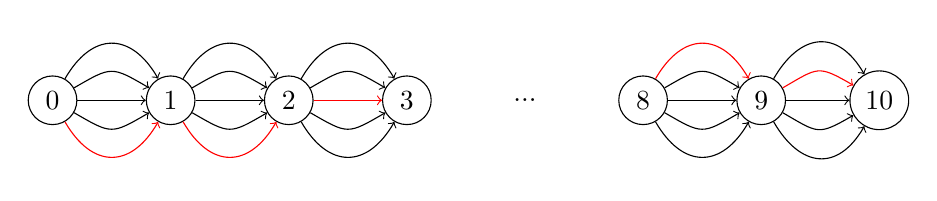
\begin{tikzpicture}[node distance={15mm}, main/.style = {circle}]
        \node[main,draw] (0) {$0$};
        \node[main,draw] (1) [right of=0] {$1$};
        \node[main,draw] (2) [right of=1] {$2$};
        \node[main,draw] (3) [right of=2] {$3$};
        \node[main  ] (...) [right of=3] {$...$};
        \node[main,draw] (8) [right of=...] {$8$};
        \node[main,draw] (9) [right of=8] {$9$};
        \node[main,draw] (10) [right of=9] {$10$};

        \foreach \m in {0,1,2,3}{
            \draw[->] (0) to [out=60-30*\m,in=120+30*\m,looseness=1.5] (1);
        }

        \draw[red, ->] (0) to [out=-60,in=240,looseness=1.5] (1);

        \foreach \m in {0,1,2,3}{
            \draw[->] (1) to [out=60-30*\m,in=120+30*\m,looseness=1.5] (2);
        }

        \draw[red, ->] (1) to [out=-60,in=240,looseness=1.5] (2);

        \foreach \m in {0,1,3,4}{
            \draw[->] (2) to [out=60-30*\m,in=120+30*\m,looseness=1.5] (3);
        }

        \draw[red, ->] (2) to [out=0,in=180,looseness=1.5] (3);
        
        \foreach \m in {1,2,3,4}{
            \draw[->] (8) to [out=60-30*\m,in=120+30*\m,looseness=1.5] (9);
        }

        \draw[red, ->] (8) to [out=60,in=120,looseness=1.5] (9);
        
        \foreach \m in {0,2,3,4}{
            \draw[->] (9) to [out=60-30*\m,in=120+30*\m,looseness=1.5] (10);
        }

        \draw[red, ->] (9) to [out=30,in=150,looseness=1.5] (10);
    \end{tikzpicture} 
\end{center}



Qui donne donc cette répartition :

\begin{table}[!h]
    \centering
    \begin{tabular}{|c|c|c|c|c|c|c|}
        \hline
        Jour  & 1    & 2     & 3       & 4 & 5    & Fitness \\
        \hline
        Cours & 8, 9 & 5, 10 & 4, 6, 7 & 3 & 1, 2 & 10      \\
        \hline
    \end{tabular}
    \caption{Répartition de l'emploi du temps de la meilleure fourmi à la génération 2}\label{tab:fourmi-finale}
\end{table}

On a réussi à atteindre une solution pour laquelle la fitness est maximale.


\subsection{Retour critique}\label{subsec:retour-critique}

Comme vu plus haut, la méthode de la colonie de fourmis ne se prête pas particulièrement à la résolution de ce genre de problème.
Bien que nous finissions par trouver une solution dont la fitness est maximale, il s'agit vraisemblablement plus de hasard que d'une réelle efficacité de la méthode.

Le principal obstacle à la conception d'un algorithme de colonie de fourmis efficace pour résoudre ce problème est due à la nature de problème d'affectation de notre problème.

Étant donné qu'aucun \og chemin \fg{} de l'arbre n'est intrinsèquement meilleur qu'un autre, la qualité de chaque chemin dépendant des chemins empruntés précédemment, les phéromones se révèlent peu utiles dans la découverte d'une solution optimale.